\documentclass[simplex.tex]{subfiles}
% NO NEED TO INPUT PREAMBLES HERE
% packages are inherited; you can compile this on its own
\begin{document}
\subsection{Network Dependence Test via Diffusion Maps and MGC} 
Deciphering the association between network structures and corresponding nodal attributes of interest is a core problem in network science. We propose a new nonparametric procedure for testing dependence between network topology and nodal attributes, via diffusion maps and \texttt{MGC}. Specifically, under an exchangeable graph, we verify that the diffusion maps provide a set of conditionally independent multivariate coordinates for the nodes, which can be combined with \texttt{MGC} (or in general, any distance-based correlation measures) to yield consistent statistic for network dependence testing. Moreover, our method is computationally inexpensive and robust against parameter mis-specifications, very efficient in capturing a wide variety of nonlinear and high-dimensional relationships, and readily extend-able to testing independence between two graphs. 

Figure~\ref{fig:threeSBM} illustrates the advantage of the proposed method on testing dependency between two graphs. The graphs are simulated by the random dot product graph, with the underlying latent variables being related by a quadratic function. By repeatedly generating dependent sample graphs, the testing power equals the percentage of rejection of the independence hypothesis. Although all methods are consistent (having power $1$ as number of vertices increases), the proposed approach using \texttt{MGC} is able to achieve perfect testing power at a very small size, which is significantly better than other benchmarks.

\begin{figure}[h!]
\begin{cframed}
		\centering
		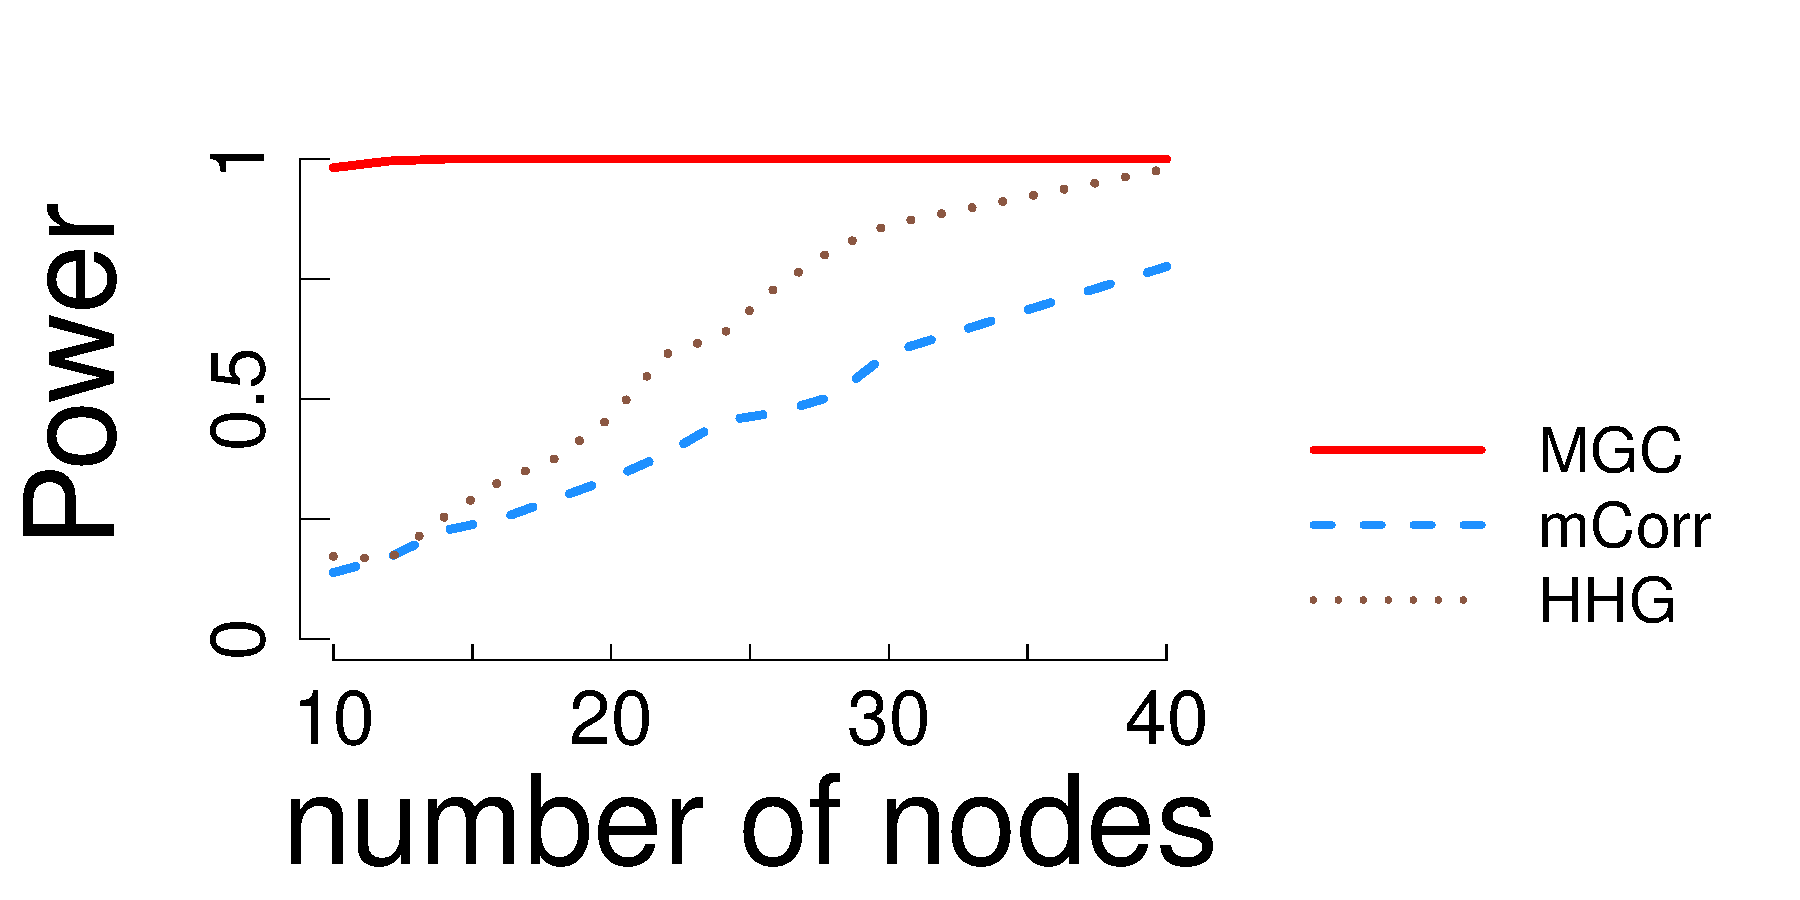
\includegraphics[width=0.7\textwidth]{../../figs/twoGraphs1.pdf}
		\caption{The power curve with respect to increasing number of vertices for the two-graph dependency testing simulation. The proposed approach quickly attains perfect power at a very small vertex size, while other benchmarks often require a much larger graph for perfect testing. }
		\label{fig:threeSBM}
		\end{cframed}
\end{figure}

An early draft is recently awarded the Best Student Paper Awards by the American Statistical Association Nonparametric Statistics Section, which will be presented in a special section in the Joint Statistical Meeting this year. We collected and addressed feedback from experts in graph inference, and submitted the complete manuscript this month.
%
\end{document}
